\section{Knowledge Graphs}
\label{cha:foundations_basics_kb}
This section provides a general overview of Knowledge Graphs.  The section contains three main subsections. In the first subsection, formal definitions of knowledge graphs and relevant details are given. In the second subsection, the most prominent open knowledge graphs are introduced. Finally, the last subsection briefly discusses the Linked Open Data.
\subsection{Definitions and Preliminaries}
The "\textit{knowledge graph}" phrase has been used in various contexts in literature at least since  1972~\cite{hogan2020knowledge}. However, after the announcement of the Google Knowledge Graph in 2012, the representation of knowledge in a graph-based form has attracted significant attention across industry and academia~\cite{DBLP:journals/semweb/Paulheim17}. Soon after the announcement of the Google Knowledge Graph many other companies from industry, e.g., Facebook, LinkedIn, IBM, Amazon, etc. focused on the development and improvement of their knowledge graphs as well. Besides, there has been a considerable amount of study on knowledge graphs, and many scientific literatures have been published~\cite{hogan2020knowledge,DBLP:journals/semweb/Paulheim17,def_of_KGs_16,farber2015comparative}. The most well-known freely accessible knowledge graphs are DBpedia, Wikidata, Freebase, etc. and the ones not openly available are Google, LinkedIn, Airbnb, etc.

Given that knowledge graphs are drawing more attention especially after the announcement of the Google Knowledge Graph, different definitions have been proposed to describe them~\cite{hogan2020knowledge}. In fact some of the definitions conflict with each other~\cite{def_of_KGs_16}. Here we present some of the most recent and prominent definitions as follows:% the term has been used widely . After that several gained more attention from Industry  Facebook eg. and academia  work on creation refinemment and so on.
%Moreover the term KG has been used refering ... by google, and currently used to refer to DBpedia... however there is still no common def of it however the following
\theoremstyle{definition}
\begin{definition}{(Knowledge Graph):\\}
\textit{"A knowledge graph is a semi-structured data model characterized by three components: (i) a ground extensional component, that is, a set of relational constructs for schema and data (which can be effectively modeled as graphs or generalizations thereof); (ii) an intensional component, that is, a set of inference rules over the constructs of the ground extensional component; (iii) a derived extensional component that can be produced as the result of the application of the inference rules over the ground extensional component (with the so-called "reasoning" process)."}~\cite{DBLP:conf/icde/BellomariniFGS19}
\end{definition}
\begin{definition}{(Knowledge Graph):\\}
\textit{“A knowledge graph mainly describes real world entities and their interrelations, organized in a graph; defines possible classes and relations of entities in a schema; allows for potentially interrelating arbitrary entities with each other; covers various topical domains."}~\cite{DBLP:journals/semweb/Paulheim17}
\end{definition}
\theoremstyle{definition}
\begin{definition}{(Knowledge Graph):\\}
\textit{“A knowledge graph acquires and integrates information into an ontology and applies a reasoner to derive new knowledge."}~\cite{def_of_KGs_16}
\end{definition}
\theoremstyle{definition}
\begin{figure*}[t]
 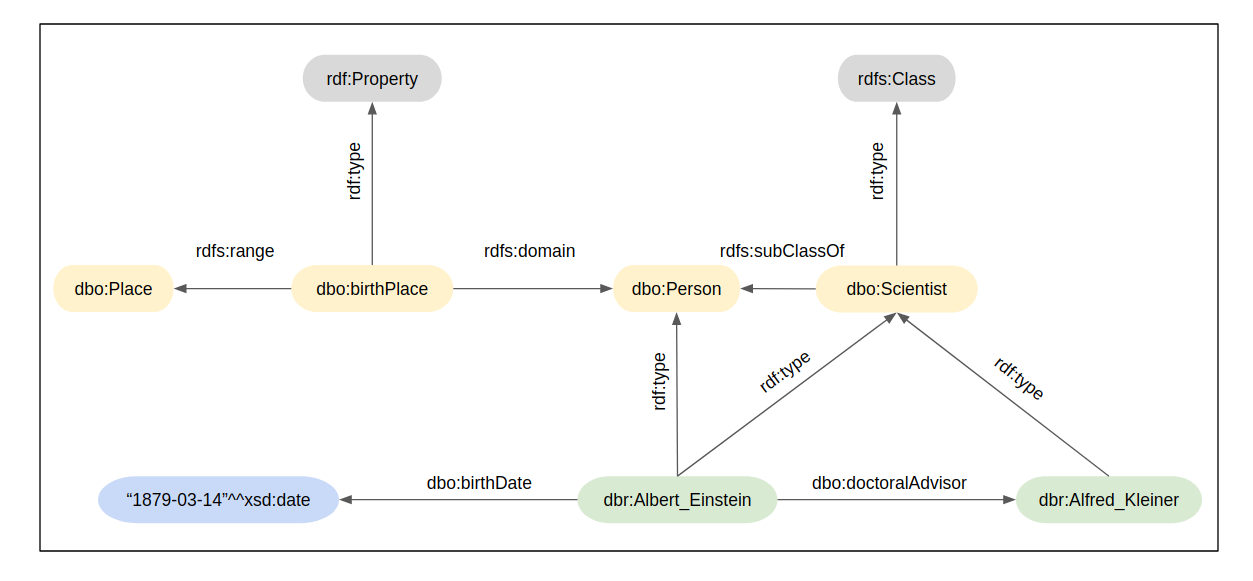
\includegraphics[width=\linewidth]{Figures/sec_KGs_RDF_graph.png}
 \caption{Example of a simple RDF graph}
 \label{fig:rdf_simple_graph}
\end{figure*} 

\theoremstyle{definition}
\begin{definition}{(Knowledge Graph):\\}
\textit{Different than the aforementioned definitions,~\textcite{DBLP:journals/semweb/FarberBMR18} gives the formal definition of a knowledge graph as an RDF graph. "An RDF graph consists of a set of RDF triples (cf. Definition~\ref{}) where each RDF triple \texttt{(s,p,o)} is an ordered set of the following
RDF terms: a subject \texttt{$\textit{s}\in\textit{U}$} $\cup$\texttt{$\textit{B}$}, a predicate \texttt{$\textit{p}\in\textit{U}$}, and an object \texttt{$\textit{U}$} $\cup$  \texttt{$\textit{B}$} $\cup$ \texttt{$\textit{L}$}. An RDF term is either a URI \texttt{$\textit{u}\in\textit{U}$}, a blank node \texttt{$\textit{b}\in\textit{B}$}, or a literal \texttt{$\textit{l}\in\textit{L}$}. \texttt{$\textit{U}$},  \texttt{$\textit{B}$} and \texttt{$\textit{L}$} are pairwise disjoint".}~\cite{DBLP:journals/semweb/FarberBMR18}
\end{definition} \todo{ask: if is it sufficient}
\theoremstyle{definition}
%\todo{footnote url}
%\todo{text font tt}
Knowledge graphs have been utilized in many real world information systems which require to leverage a structured, diverse, large-scale collection of data~\cite{DBLP:journals/semweb/Paulheim17,hogan2020knowledge}, e.g., the Google Knowledge Graph plays a very important role for enhancing the search engine results.  Besides the industry, knowledge graphs have been extensively utilized in various research areas (e.g., artificial intelligence) in academia. Moreover, the idea of leveraging structured knowledge, i.e., machine understandable knowledge by intelligent systems has been a goal of artificial intelligence research for decades~\cite{DBLP:journals/semweb/Paulheim17}. %Knowledge Graphs employ a graph-based form to represent knowledge, which can be domain specific such as facts about chemical interactions or domain independent. 

Furthermore, in the \textit{Semantic Web} community the term knowledge graph is also used to refer to the Semantic Web Knowledge Bases such as DBpedia, Wikidata, YAGO, etc.~\cite{DBLP:journals/semweb/Paulheim17} To facilitate the discussion, first we give the definition of the Semantic Web which was proposed by Tim Berners-Lee et al. as "\textit{A new form of web content that is meaningful to computers}'', in 2001. Since then the fundamentals of the Semantic Web have been based on the idea of representing knowledge in a structured and machine understandable way. Today, knowledge bases are one of the most essential components of the Semantic Web.
They employ a graph-based form to represent knowledge, which can be domain specific such as facts about chemical interactions or domain independent. The facts in knowledge bases are modeled by directed edge-labeled graphs as shown in Figure~\ref{fig:rdf_simple_graph}. Such graphs consist of a set of nodes such as \texttt{dbr:Albert\_Einstein, dbo:Scientist} and directed-labeled edges between those nodes such as \texttt{rdf:type, rdfs:subClassOf}. 
\begin{minipage}{\textwidth}
\begin{lstlisting} [caption={RDF document in turtle serialization},label=listing_rdf_serialization]

@prefix rdf: <http://www.w3.org/1999/02/22-rdf-syntax-ns#> .
@prefix rdfs: <http://www.w3.org/2000/01/rdf-schema#> .
@prefix xsd: <http://www.w3.org/2001/XMLSchema#> .
@prefix dbo: <http://dbpedia.org/ontology/> .
@prefix dbr: <http://dbpedia.org/resource/> .

dbo:birthPlace	rdfs:range	dbo:Place .
dbo:birthPlace	rdfs:domain	dbo:Person .
dbo:birthPlace	rdf:type	rdf:Property .

dbo:Scientist	rdf:type	rdfs:Class .
dbo:Scientist	rdf:subClassOf	dbo:Person .

dbr:Albert_Einstein	dbo:birthDate	"1879-03-14"^^xsd:date .
dbr:Albert_Einstein	rdf:type	dbo:Person .
dbr:Albert_Einstein	rdf:type	dbo:Scientist .
dbr:Albert_Einstein	dbo:doctoralAdvisor	dbr:Alfred_Kleiner .
\end{lstlisting}
\end{minipage}\\\\


The Semantic Web knowledge bases follow standardized data modeling formats which facilitate the knowledge exchange. These standards include but not limited to \textit{Resource Description Framework} (RDF),  \textit{Resource Description Framework Schema} (RDFS) which is an extension of the RDF and \textit{Web Ontology Language} (OWL). The specifications of the data modeling formats are published by World Wide Web Consortium\footnote{\url{https://www.w3.org/standards/}} (W3C) that is the main international standards organization for the World Wide Web.%The Semantic Web knowledge bases follow  a standardized data model so called \textit{Resource Description Framework} (RDF) which is a formal language for describing structured knowledge. The  specifications of RDF  

The RDF standards allow to define different types of nodes in a knowledge base namely, \textit{resources} (entities on the Web) which could be anything like people, location, documents, etc., \textit{literals} that allow representing data type values such as dates, integers, etc. and \textit{blank nodes}. %which are not assigned to any identifier. 
The RDF resources are identified by unique \textit{Internationalized Resource Identifiers} (IRIs)~\cite{DBLP:journals/rfc/rfc3987} that allow identification of entities on the Web. However, blank nodes are not assigned to any identifier and thus they do not carry any additional information within a knowledge base. Instead, blank nodes can only indicate an existence of a thing. The representation of knowledge in knowledge bases is based on the idea of making statements about the resources in the form of RDF triples (\texttt{subject,  predicate, object}), where the subject could be an entity or a blank node, whereas the object could be an entity or a blank node or a literal. Note that literals can only be in an object position.
\theoremstyle{definition}
\begin{definition}{(RDF triple):\\}
\textit{Given a set of URIs U,\todo{URI or IRI check} a set of blank nodes B, and a set of literals L, an RDF triple is represented as $t=(s,p,o)\in (U \cup B) \times U \times (U \cup B \cup L)$, where $s$ is a subject, $p$ is a predicate and $o$ is an object.}
\end{definition}
\theoremstyle{definition}


\theoremstyle{definition}
\begin{definition}{(Triple Pattern):\\}
\textit{"Let U, B, L be disjoint infinite sets of URIs, blank nodes, and literals, respectively. Let V be a set of variable such that $V \cap (U\cup B \cup L) = \emptyset$. A triple pattern defined as a 3-tuple $(s, p, o) \in (U\cup V) \times (U\cup V)\times (L\cup U \cup V)$, where the components subject, predicate and object correspond to RDF terms or variables."}~\cite{DBLP:phd/dnb/Deibe18}.
\end{definition}
\theoremstyle{definition}

\theoremstyle{definition}
\begin{definition}{(RDF Graph):\\}
\textit{"A finite set of RDF triples is called as RDF Graph $\mathcal{G}$ such that $\mathcal{G}=(V, E)$, where V is a set of vertices and E is a set of labeled edges.}
\end{definition}
\theoremstyle{definition}

Some of the RDF triple examples from Figure~\ref{fig:rdf_simple_graph} are \texttt{(dbr:Albert\_Einstein rdf:type dbo:Person)} and \texttt{(dbr:Alfred\_Kleiner rdf:type dbo:Scientist)}. Note that RDF's namespace abbreviated by \texttt{"rdf:"}\footnote{\url{http://www.w3.org/1999/02/22-rdf-syntax-ns#}}. There exist several serialization syntaxes to convert RDF graphs into machine readable forms such as N-triples\footnote{\url{https://www.w3.org/TR/n-triples/}}, Turtle\footnote{\url{https://www.w3.org/TR/turtle/}}, etc. Listing~\ref{listing_rdf_serialization} is the turtle serialization of the RDF graph, which is depicted in Figure~\ref{fig:rdf_simple_graph}.  Listing~\ref{listing_rdf_serialization} shows that the RDF vocabulary has been used to define resources (e.g., \texttt{dbr:Albert\_Einstein rdf:type dbo:Scientist}) and predicates (e.g., \texttt{dbo:birthPlace rdf:type dbo:Property}).

%Further, the knowledge is represented by the ontologies and 
%Figure~\ref{fig:rdf_simple_graph} illustrates that RDF can only define, i.e., assign type information to resources. 

\par Another particular RDF vocabulary is RDFS which enables the specification of schema knowledge~\cite{DBLP:books/crc/Hitzler2010}. RDFS's namespace abbreviated by \texttt{"rdfs:"}\footnote{\url{http://www.w3.org/2000/01/rdf-schema#}}. For example, the definition of domain and range of properties (e.g., (\texttt{dbo:birthPlace rdfs:domain dbo:Person}), (\texttt{dbo:birthPlace rdfs:range dbo:Place})) and hierarchical relationships, i.e, sub classes (e.g., \texttt{dbo:Scientist rdfs:subClassOf dbo:Person}), sub properties and more besides~\cite{DBLP:books/crc/Hitzler2010}. Due to capability of specifying such schema knowledge, RDFS can also be considered as an \textit{ontology language}. Let us first discuss the term \textit{ontology}. According to~\citeauthor{gruber1993translation} ontology can be defined as follows:
\begin{definition}{(Ontology):\\}
Originally,~\citeauthor{gruber1993translation}~\citeyear{gruber1993translation} defined ontology as \textit{"explicit specification of a conceptualization"}. Then, an ontology defined as "formal specification of a shared conceptualization" by bla in 1997\todo{add ref}. Finally, blabla merged these two definiations and defined an ontology as \textit{"formal, explicit specification of a shared conceptualization"}. Today, the latter definition is the one which is most commonly accepted and used.
\end{definition}
In this definition, \textit{conceptualization} implies that existing of an abstract model of a certain domain which contains identified relevant concepts and their relations. \textit{Explicit} denotes that meaning of all concepts must be defined explicitly. \textit{Shared} stands for consensus about the ontology and \textit{formal} refers to machine readability and understandability. It should be noted that each RDFS document is also an RDF document.

%Further it also defines the domain and range of properties. subclasses, subproperties, domains, and ranges amongst the classes and properties used in an RDF graph. 

%Note that each RDFS document is also an RDF document.
Figure~\ref{fig:rdf_simple_graph} illustrates that the simple ontologies can be modeled by RDF(S), however, for modeling more complex representations of knowledge the Web Ontology Language (OWL) is being used. OWL is based on formal logic and supports much greater expressiveness than RDF(S). Further, it allows logical reasoning on the knowledge and thus enables to deduce implicit knowledge which is not explicitly modeled. There exist different flavours of OWL2 which is the last version OWL and based on description logic, i.e., OWL2 EL, OWL2 RL, OWL2 QL, OWL2 DL, OWL2 Full. Each of these species of OWL2 has different level of expressivity. OWL2 DL is more expressive than OWL2 EL, OWL2 RL and OWL2 QL and less expressive than OWL2 Full.
In other words, OWL2 DL is the expressive and decidble version of OWL. Therefore, in this section we focus on OWL2 DL.

OWL2 standards which are specified by World Wide Web Consortium allow to define class expressions (e.g., conjunction, disjunction), properties, class and property axioms, and facts. Moreover, OWL supports RDF syntax therefore, similar to RDF(S) documents, each OWL document in RDF syntax is also an RDF document. OWL's name space is \\<http://www.w3.org/2002/07/owl\#> and abbreviated by "owl:". Further, the OWL axioms expressed in terms of\\ 
\begin{outline}
\1 \textbf{Classes.} OWL classes are comparable with RDF(S) classes. There exist two predefined classes in OWL namely, \texttt{owl:Thing} whose member is all individuals and \texttt{owl:Nothing} which is an empty class, i.e., it does not contain any individual. Definition of a class as follows: 
    \2 \texttt{:Wine rdf:type owl:Class.}  
 \1 \textbf{Individuals.} OWL individuals can be defined in two different ways, namely via class membership which is comparable with RDF(S) class instances and without a class membership.
\2 \texttt{:RoseWine rdf:type :Wine .}
\2 \texttt{:Beer rdf:type owl:NamedIndividual .}
\1 \textbf{Properties.} OWL allows definition of two types of properties, i.e., object properties and datatype properties and they are comparable with RDF(S) properties. 
\2 \textbf{Object Properties.} Object Properties of OWL have classes as domain and range.
\3 \texttt{:pairWith rdf:type owl:ObjectProperty ;}\\
\hspace*{2.2cm}      \texttt{rdfs:domain owl:Thing ;}\\
\hspace*{2.2cm}        \texttt{rdfs:range  :Seafood .}
\2 \textbf{Datatype Properties.} Datatype Properties of OWL have datatypes as range.
\3 \texttt{:color rdf:type owl:ObjectProperty ;}\\
\hspace*{1.6cm}\texttt{rdfs:domain owl:Thing ;}\\
\hspace*{1.6cm}\texttt{rdfs:range  xsd:date . }
\end{outline} 
%For the sake of consistency, in the following the turtle serialization(cf. Listing~\ref{listing_rdf_serialization}) of OWL2 is used in the examples of OWL axioms.
\noindent Obviously, it is also possible to define much more expressive facts with OWL such as logical class constructions, property restrictions,etc. More details about OWL can be found  in~\cite{DBLP:books/crc/Hitzler2010}.
% \begin{figure*}[t]
%  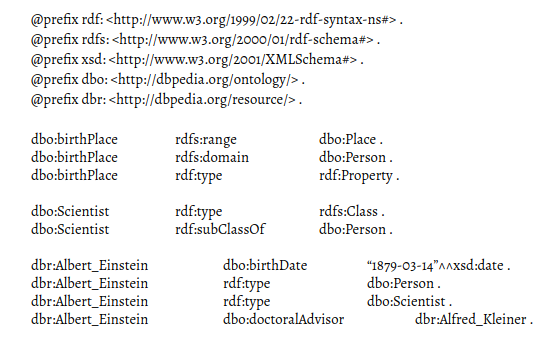
\includegraphics[width=\linewidth]{Figures/sec_KGs_RDF_turtle_serialization.png}
%  \caption{RDF document in turtle serialization}
%  \label{fig:architecture}
% \end{figure*}
\subsection{Open Knowledge Graphs} 
Open knowledge graphs are openly available and freely usable. There are different ways of constructing open knowledge graphs, i.e, they can be curated by a small group of people or crowd sourced by a large group of people or created by utilizing automatic or semi-automatic methods~\cite{DBLP:journals/semweb/Paulheim17}. In the following we give the example of knowledge bases which have been built by different methods:\\
\begin{itemize}
\item \textbf{Cyc and OpenCyc~\cite{DBLP:journals/cacm/Lenat95}.} Cyc is one of the oldest curated knowledge bases of common sense which is developed and maintained by the CyCorp company starting in 1984. The artificial intelligent project Cyc, represents millions of common sense facts. For example:
\begin{itemize}
\item"You have to be awake to eat.", 
\item"You cannot remember events that have not happened yet.".
\end{itemize}
Cyc aims to be served as a structured data source especially to the artificial intelligence based applications such as information retrieval, speech recognition, etc.~\cite{DBLP:journals/cacm/Lenat95}
%The domain of CYc is all of human consensus reality, such as thecommon sense  
A small version of Cyc, so called OpenCyc has been made publicly available in order to serve as a great data source especially, for artificial intelligence researchers. Further, there used to be an existing Semantic Web endpoint to OpenCyc\todo{tell that you are reporting the numbers from a published paper}
\todo{check numbers}
, which also contained links to other Linked Open Data\footnote{\url{https://lod-cloud.net/}} datasets such as DBpedia. The 2012 version of OpenCyc contains approximately 120,000 instances and 2.5 million facts defined for those instances and its schema consists of approximately 45,000 type hierarchy, and 19,000 possible relations~\cite{DBLP:journals/semweb/Paulheim17}. The CyCorp company, the developer of OpenCyc, has stopped online support for its knowledge base since March 2017.\\

\item \textbf{WordNet~\cite{fellbaum98wordnet}.} WordNet is a large lexical knowledge base which represents semantic relations between words for the English language. It is created in the Cognitive Science Laboratory of Princeton University staring in 1985. WordNet includes the lexical categories of different types of words, i.e., nouns, verbs, adjectives and adverbs. The words that are from the same lexical category grouped into unordered sets of cognitive synonyms, called \textit{synsets}. Synsets are interlinked by the means of semantic links such as hyperonymy, meronymy. This knowledge graph can be navigated easily with the browser. WordNet is publicly available and can be downloaded freely. The 3.0 version of WordNet contains in total 117,659 synsets for 155,287 unique strings,including 82,115 synsets for 117,798 nouns, 13,767 synsets for 11,529 verbs, 18,156 synsets for 21,479 adjectives, 3,621 synsets for 4,481 adverbs, as well as 206,941 word-sense pairs,including 146,312 for nouns, 25,047 for verbs, 30,002 for adjectives, 5,580 for adverbs.\\
\todo{check the numbers}

\item \textbf{Freebase~\cite{DBLP:conf/sigmod/BollackerEPST08}.} Freebase is a public knowledge base which is created through crowd sourcing by the announcement of American software company Metaweb in March 2007. In contrast to other curated knowledge bases, e.g., Cyc, which required more than 900 person years to create~\cite{DBLP:journals/semweb/Paulheim17}, Freebase provided an interface to the public editors.  Thereby, the editors could directly contribute to the knowledge base by editing structured data with schema templates. Besides the contribution of the editors, the knowledge from Wikipedia has been integrated to Freebase~\cite{farber2015comparative}. In 2010, Freebase acquired by Google and on August 31, 2016, it was completely shut down. The last version of Free-base contains roughly 50 million entities and 3 billion facts. The Freebase schema comprises roughly 27,000 entity types and 38,000 relations~\cite{DBLP:journals/semweb/Paulheim17}.\\

\item \textbf{Wikidata~\cite{DBLP:journals/cacm/VrandecicK14}.} Wikidata is a collaboratively edited knowledge base by the community and it is operated by the Wikimedia foundation. Wikidata has been extensively exploited as a main data source in a wide range of information system applications, especially in the Semantic Web community. Unlike aforementioned KBs, Wikidata does not only contain facts but also the source of the facts so that the validity of facts can be approved. Moreover, after the shut down of Freebase, its data moved to Wikidata. To date, Wikidata contains roughly 83,343,004 instances\footnote{\url{https://www.wikidata.org/wiki/Wikidata:Main_Page}} and 1,036,340,466 million statements\footnote{\url{http://tools.wmflabs.org/wikidata-todo/stats.php}}. Its schema defines roughly 7,450 relations\footnote{\url{https://www.wikidata.org/w/index.php?title=Special:ListProperties}}.\\

\item \textbf{DBpedia~\cite{DBLP:conf/semweb/AuerBKLCI07}.} DBpedia is the most popular KG in Linked Open Data cloud and it was initiated by the researchers from the Free University of Berlin and the University of Leipzig, in collaboration with OpenLink Software~\cite{farber2015comparative}. Unlike the aforementioned KBs, DBpedia has been created by automatically extracting structured and multilingual knowledge from Wikipedia, i.e., Wikipedia infoboxes. The types of infoboxes in Wikipedia are mapped to the DBpedia ontology (i.e., DBpedia Classes), further the attributes of these info boxes corresponds to the properties in DBpedia ontology~\cite{DBLP:journals/semweb/Paulheim17}. Similar to Wikidata, DBpedia has been extensively utilized in various research fields of the Semantic Web. The most recent version of the main DBpedia (i.e., DBpedia 2016-10, extracted from the English Wikipedia based on dumps from October 2016) contains 6.6M entities\footnote{\url{https://wiki.dbpedia.org/develop/datasets/dbpedia-version-2016-10}}, 13 billion facts (RDF triples), and the schema comprises 760 classes, 1,105 object properties, 1,622 datatype properties.\\

\item \textbf{YAGO~\cite{suchanek2007yago}.} Like DBpedia, YAGO is also extracted from Wikipedia and developed at the Max Planck Institute for Computer Science in Saarbrücken since 2007~\cite{farber2015comparative}. In contrast to DBpedia, YAGO comprises information not only from Wikipedia (e.g., categories, redirects, infoboxes) but also WordNet (e.g., synsets, hyponymy), GeoNames~\cite{farber2015comparative,fabian2007yago}. Further, DBpedia creates different interlinked KBs for each Wikipedia language edition (e.g., English, German, etc.), however, YAGO aims to build fusion of knowledge which extracted from various Wikipedia language editions. The latest release of YAGO, i.e., YAGO3, contains approximately 4.5 million entities and 24 million facts about such  entities  in  10  languages.   The  schema  comprises  488,496  classes  and  77 manually defined relations~\cite{DBLP:conf/cidr/MahdisoltaniBS15}.\\
 
\item \textbf{NELL~\cite{DBLP:conf/wsdm/CarlsonBWHM10}.} Never Ending Language Learning\footnote{\url{http://rtw.ml.cmu.edu/rtw/}} (NELL) is a project developed by a research team at Carnegie Mellon University since January 2010. Unlike DBpedia and YAGO which utilizes semi-structured content (e.g, Wikipedia Infoboxes)  as a base, NELL designed to exploit unstructured data to extract meaningful knowledge. In other words, the project attempts to conduct two main tasks everyday.
First, it attempts to extract facts from text found in hundreds of millions of web pages (e.g., servedWith(tea, biscuits)).
Second, it attempts to improve its fact extracting capability, so that next time it can extract more facts from the web, more accurately. Each extracted fact has a weight which reflects the confidence of it. The system is still running today and has been extending its knowledge base since the project has developed. So far, NELL has accumulated over 50 million candidate beliefs by reading the web and 2,810,379 of these beliefs are in high confidence. On NELL website, only the beliefs that has the high confidence are displayed. 
\end{itemize}\vspace{0.5cm}
\noindent Most of the open knowledge bases contain links to other RDF data sources. By doing so, users can navigate between
different data sources by following RDF links. Hence, the Semantic Web aims to make meaningful links between publicly available RDF data sources (e.g, DBpedia, Wikidata, etc.) to enable persons and machines to explore \textit{Linked Open Data} freely. In the following let us  briefly discuss the phrase \textit{Linked Open Data}.\\

\subsection{Linked Open Data}
%\noindent \textbf{Linked Open Data (LOD).}
Linked Open Data (LOD) refers to publicly available RDF data which is identified via URI and accessible via HTTP on the Web. Further, those RDF datasets are linked to other datasets via URI. Accordingly, the Linked Open Data project aims to identify datasets that are available under open licenses, re-publish
these in RDF on the Web and interlink them with each other~\cite{DBLP:conf/www/BizerHIB08}. \\

\noindent The principles of Linked Data were first outlined by Berners-Lee in 2006:
\begin{itemize}
\item Use URIs as names for things.
\item Use HTTP URIs so that people can look up those names.
\item When someone looks up a URI, provide useful information, using the standards (e.g. RDF).
\item Include links to other URIs, so that they can discover more
things.
\end{itemize}
The four rules provide broad guidance on which publishing RDF data can be based. LOD can be accessed using traditional HTML
browsers and users can easily explore and navigate between different data sources.

The network of publicly available RDF datasets that are in concordance with linked data principles has grown globally. As of April 2017, the number of publicly available RDF datasets is 9960 and it contains roughly more than 149 billion facts and roughly more than 800 million links.%\todo{check the numbers} 
The visualization of interlinked RDF datasets which is referred to as \textit{Linked Open Data Cloud\footnote{\url{https://lod-cloud.net/}}} has been  created by~\citeauthor{LOD_cloud}.  Figure~\ref{fig:lod_cloud} illustrates the evolution of the LOD cloud from its beginning in 2007 until 2019. \todo{tell that each color represents a different domain such as bla bla} 

Each node in the networks represents one dataset. As of March 2019, the huge network contains 1,239 datasets with 16,147 links. Moreover, DBpedia has been one of the most popular datasets in these networks across the years. 
%Semantic web is about making meaningful links between heterogeneous data sources to enable persons and machines to explore a "web of data" 
\newpage
%\vspace{-15cm}
\begin{figure}[t]
%\centering
\captionsetup{justification=centering, margin={0cm,0.5cm}}
\begin{minipage}{.5\textwidth}
  \centering
  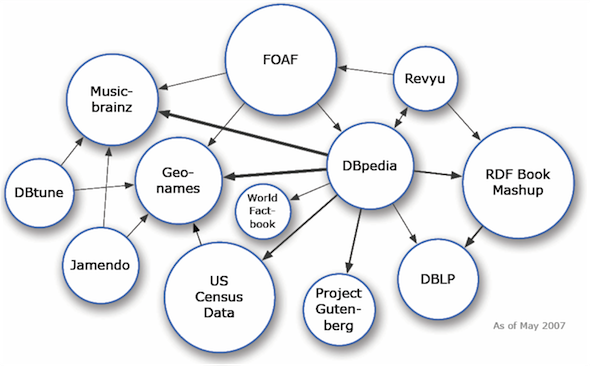
\includegraphics[width=\linewidth]{Figures/LOD/lod-cloud_2007.png}
  \caption*{March 2007 (12 datasets)}
  \label{fig:test1}
\end{minipage}%
\hspace{0.5cm}
\begin{minipage}{.5\textwidth}
  %\centering
  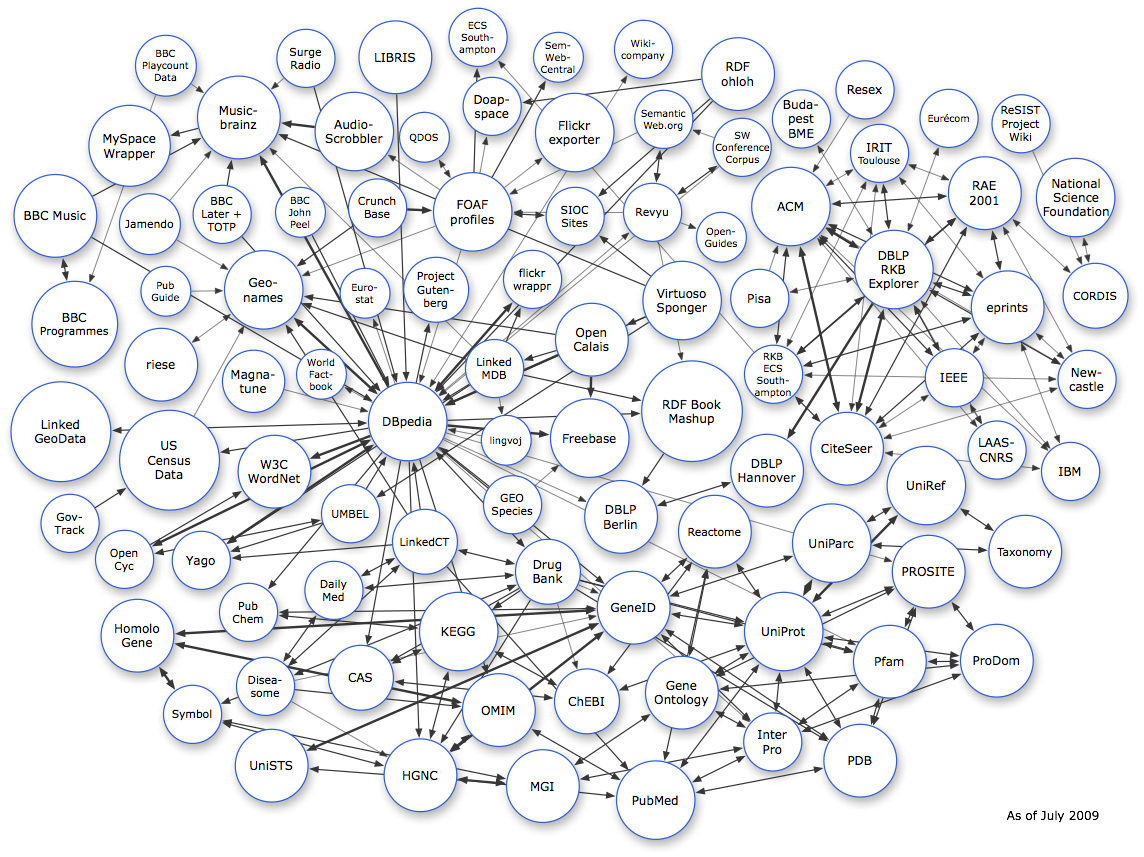
\includegraphics[width=\linewidth]{Figures/LOD/lod-cloud_2009.png}
  \caption*{July 2009 (95 datasets)}
  \label{fig:test2}
\end{minipage}
\end{figure}
\vspace{5cm}

\vspace{10cm}
\vspace{5cm}
\begin{figure}
\centering
\captionsetup{justification=centering, margin={0cm,0.5cm}}
\begin{minipage}{.5\textwidth}
  \centering
  \includegraphics[width=\linewidth]{Figures/LOD/lod-cloud_2014.png}
  \caption*{March 2007 (12 datasets)}
  \label{fig:test1}
\end{minipage}%
\begin{minipage}{.5\textwidth}
  \centering
  \includegraphics[width=\linewidth]{Figures/LOD/lod-cloud_2017.png}
  \caption*{July 2009 (95 datasets)}
  \label{fig:test2}
\end{minipage}
\end{figure}


%\input{Figures/fig_deneme}
\clearpage

\begin{figure}[t!]
\centering
\captionsetup{justification=centering,margin=2cm}
 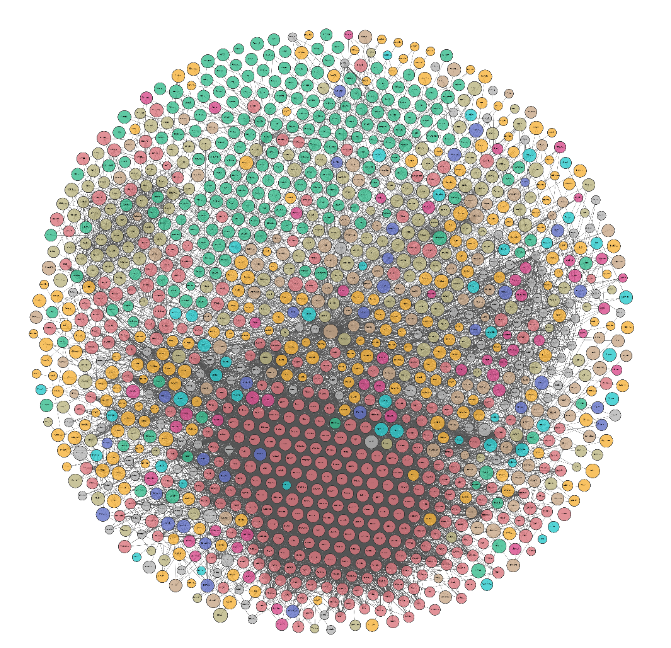
\includegraphics[height=9cm,width=9cm]{Figures/LOD/fig_LOD_2019_clean.png}
 \caption{March 2019 (1,239 datasets)}
 \label{fig:lod_cloud}
\end{figure}


%\clearpage
